\documentclass[10pt,journal]{IEEEtran}

% *** GRAPHICS RELATED PACKAGES ***
%
\ifCLASSINFOpdf
  \usepackage[pdftex]{graphicx}
  % declare the path(s) where your graphic files are
  \graphicspath{{../pdf/}{../jpeg/}}

  \DeclareGraphicsExtensions{.pdf,.jpeg,.png}
\else
  % or other class option (dvipsone, dvipdf, if not using dvips). graphicx
  % will default to the driver specified in the system graphics.cfg if no
  % driver is specified.
  % \usepackage[dvips]{graphicx}
  % declare the path(s) where your graphic files are
  % \graphicspath{{../eps/}}
  % and their extensions so you won't have to specify these with
  % every instance of \includegraphics
  % \DeclareGraphicsExtensions{.eps}
\fi


\usepackage[utf8]{inputenc}
\usepackage[portuguese]{babel}
\usepackage{amsfonts}
\usepackage{amssymb}
\usepackage{makeidx}
\usepackage[pdftex]{hyperref}
\usepackage{indentfirst}
\usepackage{pdfpages}
\usepackage{enumerate}
\usepackage{amsmath}
\usepackage{algorithmic}
\usepackage{array}
\usepackage{url}
\usepackage{cite}
\usepackage[nottoc]{tocbibind}
\usepackage{lipsum}
\usepackage{booktabs}
\usepackage{tikz}
\usepackage[justification=centering]{caption}
\usepackage{hyperref}
\usepackage{mathptmx} 

\graphicspath{{imagens/}}

\renewcommand\IEEEkeywordsname{Palavras-chave}

\begin{document}

\title{UM APLICATIVO CONTADOR DE MOEDAS UTILIZANDO OPENCV}

\author{\IEEEauthorblockN{Denis Ricardo da Silva Medeiros}
\IEEEauthorblockA{Departamento de Engenharia de Computação\\
		Universidade Federal do Rio Grande do Norte\\
		Natal, Rio Grande do Norte (84) 3342-2231\\
		Email: dnsricardo@gmail.com}
	\and \\
	\IEEEauthorblockN{Pedro Henrique de Medeiros Leite}
	\IEEEauthorblockA{Departamento de Enegenharia Elétrica\\
		Natal, Rio Grande do Norte (84) 3215-3731\\
		Email: pedrohenriquedemedeiros@gmail.com}
}

% make the title area
\maketitle

\begin{abstract}
O objetivo deste trabalho é propor uma nova estratégia de detecção e classificação de moedas em imagens digitais, através do desenvolvimento de um aplicativo que seja capaz de contar dinheiro utilizando uma câmera digital, como a de um telefone celular, por exemplo. Para conseguir isso, são aplicadas várias técnicas de processamento digital de imagens durante a busca por moedas e também de inteligência artificial para sua classificação, mais precisamente com redes neurais artificiais (RNAs). Durantes os experimentos, o aplicativo final foi calibrado com 60 e validado com 20 moedas, conseguindo atingir 100\% de acerto. Por fim, o aplicativo contador conseguiu realizar com sucesso a contagem de dinheiro de um conjunto de moedas, atingindo o objetivo para o qual ele foi proposto. 
\end{abstract}

\begin{IEEEkeywords}
Processamento digital de imagem, moedas, classificação, contagem, redes neurais artificiais.
\end{IEEEkeywords}


% For peer review papers, you can put extra information on the cover
% page as needed:
% \ifCLASSOPTIONpeerreview
% \begin{center} \bfseries EDICS Category: 3-BBND \end{center}
% \fi
%
% For peerreview papers, this IEEEtran command inserts a page break and
% creates the second title. It will be ignored for other modes.
\section{Introdução}
\label{sec:introducao}

No dia a dia do consumidor, moedas são formas indispensáveis de se fazer pequenas compras, dar ou facilitar o troco em supermercados ou até mesmo para troca em cédulas. Dessa forma, devido ao comércio estar equipado com máquinas para o pagamento ser feito em cartão de crédito, no caso de grandes compras, ou contadores de cédulas em bancos para contagem de papel moeda, a contagem de moedas de forma automatizada para fins comerciais  muitas vezes acaba por ser negligenciado pelas pessoas.

Nesse contexto, a automatização desse processo poderia proporcionar economia de tempo e consequentemente de dinheiro para as empresas, já que contar muitas moedas pode ser um trabalho árduo e demorado. Atualmente, já existem algumas tecnologias capazes de realizar tal tarefa, em geral atuando na comparação do peso das moedas. Entretanto, tais equipamentos ainda são bastante caros e inacessíveis para pequenos e microempresários.

Com base nesse cenário, uma possibilidade para realizar o processo de contagem de moedas de uma forma simples e barata seria através de imagens capturadas por câmeras digitais, dispositivos amplamente acessíveis e presentes em telefones celulares, computadores, televisores, dentre outros. Contudo, o processamento digital de imagens contendo moedas não é simples e tem sido objeto de estudo de vários pesquisadores.

Em seu trabalho, \cite{bremananth2005new} utilizou como estratégia reconhecer os caracteres numéricos presentes nas moedas indianas como forma de identificá-las. Embora interessante, essa estratégia é falha paras as moedas de Real do Brasil, visto que um dos lados dela não possui número. Em outro trabalho, \cite{chetan2013robust} tentou realizar a identificação através de casamento de características (\textit{feature matching}), tanto das bordas quanto com do raio das moedas. Porém, pode não ser interessante para as moedas de Real, pois elas possuem tamanhos muito parecidos, variando o raio, em alguns casos, em somente 1 mm, como pode ser visto em \cite{bcb}.

Muitos dos trabalhos publicados nessa área abordam diferentes estratégias a respeito de que características das moedas serão utilizadas em sua identificação. Porém, em geral, a maioria deles utiliza como método de classificação técnicas de inteligência artificial, mais especificamente redes neurais artificiais (RNAs), em sua maioria do tipo \textit{multilayer perceptron}, como podem ser visto em \cite{bremananth2005new}, \cite{kaur2015coin}, \cite{modi2013automated} e até em trabalhos mais antigos, como em \cite{fukumi1992rotation}.

Após essa contextualização, este trabalho propõe uma nova estratégia na identificação e classificação de moedas, com o propósito de se criar um aplicativo contador de moedas de Real presentes em uma imagens obtidas por câmera digital. A ideia é que o usuário do aplicativo tire uma foto de um conjunto de moedas em uma cena padronizada e ele informe ao usuário quanto de dinheiro está presente ali. Além do próprio aplicativo contador, também serão desenvolvidos módulos auxiliares para realizar a calibração e validação do sistema principal, sendo eles o segmentador, o calibrador e o validador.

A tecnologia da classificação e identificação das moedas utilizada também será redes neurais artificiais, mas, diferente de outros trabalhos, as características a serem extraídas das moedas brasileiras tentarão tirar proveito do tamanho, das cores e de suas texturas. Por fim, como este projeto é apenas um protótipo, o aplicativo inicial será configurado para contar apenas moedas de R\$ 0,25, R\$  0,50 e R\$ 1,00.

\section{Metodologia Utilizada}
\label{sec:metologia-utilizada}

\subsection{Análise das Características das Moedas}
\label{sec:metodologia-moedas}

\begin{table*}[]
\centering
\begin{tabular}{@{}ccll@{}}
\toprule
\textbf{Valor Facial (R\$)} & \textbf{Diâmetro (mm)} & \multicolumn{1}{l}{\textbf{Bordo}} & \multicolumn{1}{l}{\textbf{Material}}                    \\ \midrule
0,01                        & 17,00                  & liso                               & Aço revestidode cobre                                    \\
0,05                        & 22,00                  & liso                               & Aço revestidode cobre                                    \\
0,10                        & 20,00                  & serrilhado                         & Aço revestidode bronze                                   \\
0,25                        & 25,00                  & serrilhado                         & Aço revestidode bronze                                   \\
0,50                        & 23,00                  & legenda                            & Aço inoxidável                                           \\
1,00                        & 27,00                  & serrilhaintermitente               & Aço inoxidável (núcleo) e aço revestido de bronze (anel) \\ \bottomrule
\end{tabular}
\caption{Detalhes das moedas de Real brasileiro}
\label{tab:moedas}
\end{table*}


A primeira etapa deste trabalho foi analisar os objetos de estudo, isto é, as moedas de Real do Brasil para decidir a melhor estratégia para identificá-las. Notou-se que elas possuem tamanhos diferentes, mas muito próximos, o que torna essa informação isolada muito sensível a erros. Por exemplo, a diferença  de raio da moeda R\$ 0,05 para a de R\$ 0,10 é de apenas 1 mm, conforme pode ser visto na Tabela \ref{tab:moedas}, com dados do Banco Central do Brasil \cite{bcb}. Notou-se, também, que elas possuem cores e texturas diferentes, dependendo da combinação de materiais com que elas são feitas. Na Figura \ref{fig:moedas-real}, é possível perceber algumas dessas características.

\begin{figure}[ht]
\centering
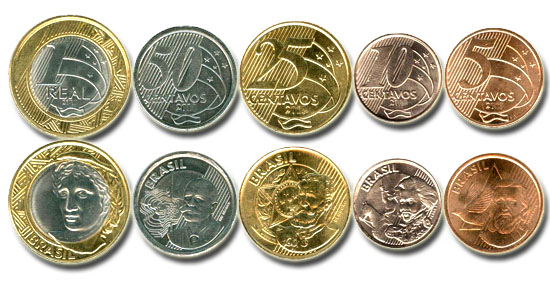
\includegraphics[width=0.5\textwidth]{moedas-real.jpg}
\caption{Todas as moedas de Real Brasileiro}
\label{fig:moedas-real}
\end{figure}


A partir dessas informações, decidiu-se que seriam utilizadas informações sobre o tamanho da imagem, para tirar proveito da diferença do diâmetro, e do material de construção, que influencia tanto na cor e na textura das moedas presentes nas imagens. Nesse caso, elas seriam utilizadas como descritores das moedas classificação, ou seja, como entradas para a rede neural artificial. 

Nessa situação, as cores são muito na diferenciação das moedas e portanto as moedas não podem ser trabalhadas em escala de cinza, pois poderia-se bastante informação útil. Assim, para uma imagem contendo uma única moeda posicionada ao centro, resultado de um processo de busca em uma imagem com várias moedas, conforme será melhor explicado adiante, com fundo branco e com seu raio tocando a borda da imagem, os seguintes elementos foram escolhidos para representá-la:

\begin{itemize}  
\item Cores da moeda: histograma da matiz da imagem. 
\item Diâmetro da moeda: largura e altura da imagem.
\item Material da moeda: características da textura da imagem.
\end{itemize}

Com isso definido, a etapa seguinte foi pensar sobre como realizar a aquisição das imagens contendo as moedas. Como uma das motivações deste projeto é a alta difusão de câmeras digitais em telefones celulares, então seria razoável que as imagens para este experimento fossem obtidas em um desses equipamentos, para manter uma compatibilidade de resolução e qualidade das fotos entre os experimentos em laboratório com o mundo real. 

Estabelecido o tipo de câmera, foi decidido também que as moedas seriam fotografadas frontalmente e deveriam estar sob algum fundo branco, como uma folha de papel A4, por exemplo, além de não ficarem sobrepostas, nem nas bordas limite da imagem. Isso porque ficaria muito difícil encontrá-las durante a etapa da localização individual das moedas em uma imagem maior, que baseia-se na busca por círculos, e também na própria classificação delas, já que perderiam-se detalhes sobre toda sua cor, textura e tamanho. 

Por fim, também fixou-se uma distância padrão entre a câmera do celular e o local onde estavam as imagens em 30 cm. Essa escolha é importante para garantir uma maior consistência na largura e altura das imagens das moedas individuais durante a classificação, pois, caso a distância de captura fosse variável, uma moeda maior poderia ser confundida com uma menor, por exemplo.

Na Figura \ref{fig:imagem-exemplo}, segue um exemplo de uma imagem atendendo aos três limites impostos acima.

\begin{figure}[ht]
\centering
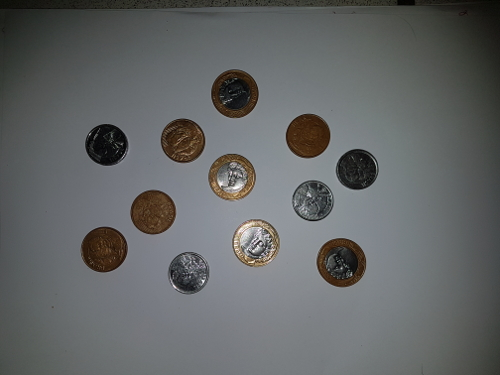
\includegraphics[width=0.5\textwidth]{completa4.jpg}
\caption{Exemplo de imagem que atendem às limitações impostas pelo projeto}
\label{fig:imagem-exemplo}
\end{figure}

Na imagem acima, também nota-se outra restrição imposta por este projeto. Nela, há apenas moedas de R\$ 0,25, R\$ 0,50 e R\$ 1,00. Isso foi necessário porque na fase de testes do aplicativo, detectou-se alguns falsos positivos entre as moedas de R\$ 0,05 R\$ 0,25, já que ambas possuem tamanho e cor semelhantes (ver Figura \ref{fig:moedas-real}). Essas falhas ocorrem, principalmente, devido às imagens obtidas através da câmera do celular serem de baixa qualidade e não conseguiam capturar pequenos detalhes cruciais na diferenciação das moedas. Logo, essas moedas foram escolhidas por serem bem diferentes entre si e por serem as de maior valor.


\subsection{Segmentação e Busca por Moedas}
\label{sec:segmentacao}

Neste momento, já se sabe que o sistema será planejado para classificar os três tipos de moedas citados anteriormente. Esta etapa consiste em separar individualmente todas as moedas que estão presentes em uma imagem maior que contém várias moedas, para que elas possam ser identificadas individualmente.

A ideia pensada aqui foi realizar uma busca por círculos na imagem. A literatura aborda várias formas de se fazer isso, sendo a transformada de Hough, provavelmente, a mais comum, como pode ser vista em \cite{ioannou1999circle}, \cite{kerbyson1995circle} e \cite{yuen1990comparative}. Outros pesquisados desenvolveram variações dessa transformada para melhorar sua eficácia e eficiência, como a sua versão adaptativa \cite{illingworth1987adaptive}, ou sua versão mais rápida e otimizada para detectar até mesmo elipses \cite{guil1997lower}.

A estratégia criada para resolver a detecção das moedas, porém, não utilizará as técnicas tradicionais baseadas na transformada de Hough, que até chegou a ser testada na fase preliminar deste projeto, mas não se mostrou completamente satisfatória. Em vez dela, foi desenvolvida uma técnica intuitiva baseando no seguinte princípio:

\begin{enumerate}
\item Procurar por contornos em uma imagem pré-processada, sendo esses candidatos a moedas.
\item Criar o menor círculo possível que consegue circundar esse contorno.
\item Comparar a área do contorno e desse círculo e verificar se ambas são semelhantes, através da comparação com um limiar pré-estabelecido.
\end{enumerate}

Combinado com essa ideia, também foi estabelecido um limiar de tamanho mínimo do raio desse círculo, pois se fosse muito pequeno certamente poderia ser algum ponto de sujeira ou ruído na imagem.

Embora essa estratégia criada pareça fácil, ela necessita de um pré-processamento bem robusto, que mantenha presente na imagem apenas contornos externos da borda externa moeda. Isso é importante até mesmo para evitar que se faça uma má detecção do contorno do círculo interno da moeda de R\$ 1,00, que poderia ser confundida com a de R\$ 0,50, por exemplo. Então, esse processamento prévio foi feito da seguinte forma:

\begin{enumerate}

\item Inicialmente, a imagem passa por um filtro gaussiano com o objetivo de suavizá-la e remover ruídos.
\item Após isso, ela é convertida para escala de cinza e passa por processo de limiarização, através do método de Otsu, com o objetivo de manter em preto o fundo da cena e em branco os objetos detectados.
\item O passo seguinte é a remoção de possíveis moedas presentes na borda, buscando remover qualquer objeto na cor branca que esteja nesse local através do algoritmo de \textit{flood fill}.
\item Adiante, é aplicado o fechamento morfológico, com o objetivo de aglutinar possíveis falhas no contorno da moeda, além de remover pequenos ruídos e contornos de dentro da moeda. Este passo é feito em quatro etapas, variando o tamanho elemento estruturante de 1 até 8 em potências de 2, de modo que o resultado final seja o que consiga detectar mais moedas.
\item Por fim, são removidos os demais resíduos remanescentes presentes dentro das moedas, através de um processo de rotulação. 
\end{enumerate}

Com esse pré-processamento, finalmente é possível aplicar a estratégia de detectar círculos descrita anteriormente. Ao fim do processo, são geradas imagens menores contendo apenas a moeda no centro, com seu raio tocando a borda da imagem.

\subsection{Classificação com Redes Neurais Artificiais}
\label{sec:metodologia-rna}


Com os descritores das imagens das moedas bem definidos na Seção \ref{sec:metodologia-moedas}, foi possível, então, planejar a rede neural artificial responsável por realizar a identificação e classificação dos três tipos de moedas: R\$ 0,25, R\$ 0,50 e R\$ 1,00. De antemão, já foi escolhido que a RNA possuiria três saídas com variação de -1 a 1, uma para cada tipo de moeda, de modo que a saída de maior valor indicasse qual a qual classe a moeda pertenceria. Por exemplo, se a primeira saída representasse a moeda de R\$ 0,25 e durante a classificação ela fosse 0.7 e as outras duas -0.5 e -0.4, então o sistema classificaria aquela moeda presente na imagem como uma moeda de R\$ 0,25.

Como entrada da rede neural, os descritores foram abstraídos da seguinte forma:

\begin{itemize}  
\item Histograma com 32 níveis da matiz da imagem.
\item Número de colunas e linhas da matriz da imagem, representando largura e altura.
\item 7 momentos invariantes da imagem convertida para escala de cinza, representando a textura da moeda.
\end{itemize}

É importante enfatizar que, antes da obtenção desse histograma, a imagem original passa por uma equalização de histograma, para distribuir melhor a iluminação da imagem. Para isso, ela é convertida de RBG para YCrCb, cujo canal Y, que representa a iluminância e é equivalente à imagem em escala de cinza, é equalizado. Ao fim, a imagem é convertida novamente para RGB. 

Com esses parâmetros, é possível montar um vetor de entrada para a RNA  de 41 elementos, sendo os 32 primeiros os níveis do histograma, os 2 próximos a altura e largura, respectivamente, e, por último, os 7 momentos invariantes da imagem contendo a moeda. Os demais ajustes da rede neural dizem respeito à sua estrutura interna e ao treinamento supervisionado. Todos os que foram aplicados no experimento foram obtidos e testados empiricamente, tentando buscar sempre uma boa precisão dos resultados quanto um bom desempenho durante o treinamento, já que esta etapa faz parte da calibração do sistema.

O diagrama da Figura \ref{fig:rna} mostra a estrutura final da rede neural artificial de múltiplas camadas utilizada nesse projeto (a entrada de valor 1 está omitida).

\tikzset{%
  every neuron/.style={
    circle,
    draw,
    minimum size=0.5cm
  },
  neuron missing/.style={
    draw=none, 
    scale=2,
    text height=0.200cm,
    execute at begin node=\color{black}$\vdots$
  },
}

\begin{figure}
\centering
\begin{tikzpicture}[x=1cm, y=1cm, >=stealth,scale=1.0]

% Definição de neurônios

\foreach \m/\l [count=\y] in {1,2,3,4,missing,5}
  \node [every neuron/.try, neuron \m/.try] (input-\m) at (0,2.5-\y) {};

\foreach \m [count=\y] in {1,2,missing,3}
  \node [every neuron/.try, neuron \m/.try ] (hiddenA-\m) at (2,2-\y*1.25) {};

\foreach \m [count=\y] in {1,2,missing,3}
  \node [every neuron/.try, neuron \m/.try ] (hiddenB-\m) at (4,2-\y*1.25) {};

\foreach \m [count=\y] in {1,2,3}
  \node [every neuron/.try, neuron \m/.try ] (output-\m) at (6,1.5-\y) {};
  
% Definição dos labels.

\foreach \l [count=\i] in {1,2,3,4,41}
  \draw [<-] (input-\i) -- ++(-1,0)
    node [above, midway] {$E \l$};

\foreach \l [count=\i] in {1,2,32}
  \node [above] at (hiddenA-\i.north) {$G \l$};
  
\foreach \l [count=\i] in {1,2,32}
  \node [above] at (hiddenB-\i.north) {$H \l$};

\foreach \l [count=\i] in {1,2,3}
  \draw [->] (output-\i) -- ++(1,0)
    node [above, midway] {$S \l$};
    
% Definição das setas.

\foreach \i in {1,...,5}
  \foreach \j in {1,...,3}
    \draw [->] (input-\i) -- (hiddenA-\j);
    
\foreach \i in {1,...,3}
  \foreach \j in {1,...,3}
    \draw [->] (hiddenA-\i) -- (hiddenB-\j);
    
\foreach \i in {1,...,3}
  \foreach \j in {1,...,3}
    \draw [->] (hiddenB-\i) -- (output-\j);

% Definição dos títulos.

%\foreach \l [count=\x from 0] in {Input, Hidden, Hidden, Ouput}
%  \node [align=center, above] at (\x*2,2) {\l \\ layer};

\node [align=center, above] at (0*2,2) {\\Camada \\ de Entrada};
\node [align=center, above] at (1*2,2) {\\Camada \\ Escondida};
\node [align=center, above] at (2*2,2) {\\Camada \\ Escondida};
\node [align=center, above] at (3*2,2) {\\Camada \\ de Saida};

\end{tikzpicture}
\caption{Diagrama da Rede Neural Artificial}
\label{fig:rna}
\end{figure}


\subsection{Tecnologias Utilizadas}
\label{sec:tecnologias-envolvidas}

O aplicativo proposto nesse projeto foi desenvolvido completamente com tecnologias livres e gratuitas, assim como também será o resultado final aqui produzido. Ele foi desenvolvido em linguagem de programação C++, com compilador GNU C++ 5.4.0, e com o apoio da biblioteca Open Source Computer Vision Library (OpenCV), versão 2.4.9. Como plataforma de desenvolvimento, de testes e execução do software final, foi utilizado o Ubuntu 16.04 LTS, em sua versão de 60 bits. Por fim, a câmera utilizada foi a de um \textit{smartphone} convencional, com resolução de 12 megapíxels.

O código fonte do projeto pode ser encontrado no Github no seguinte \textit{link}:

\url{https://github.com/PedroHenriqueMedeiros/PedroHenriqueMedeiros.github.io/tree/master/%DCA0445/src/projetofinal}

\section{Resultados}
\label{sec:resultados}

Os resultados  abaixo mostram como é o passo-a-passo de utilização dos módulos desenvolvidos neste projeto, sendo o último o principal, que realiza a contagem das moedas em si. 

\subsection{Segmentador}
\label{sec:segmentador}

O segmentador é o módulo responsável por receber como entrada uma imagem contendo várias moedas e separá-las em imagens individuais, atendendo a estratégia e os requisitos citados na Seção \ref{sec:segmentacao}. Na Figura \ref{fig:resultado-segmentador}, segue um exemplo de execução deste módulo. Tanto para este teste de execução a quanto para os seguintes foi utilizada a Figura \ref{fig:imagem-exemplo}. Nele, os parâmetros utilizados foram os seguintes:

\begin{itemize}  
\item Menor tamanho acaitável para o raio de uma moeda: 50 píxels
\item Menor relação entre a área do contorno e a do o círculo que circunda este contorno: 70\%
\end{itemize}

Os passos de pré-processamento descritos na Seção \ref{sec:segmentacao} podem ser ser resumidos nas Figuras \ref{fig:gaussiano}, \ref{fig:binaria-otsu} e \ref{fig:fechamento-buracos}. Já a estratégia de detecção de círculos pode ser percebida na Figura \ref{fig:circulos}. Todas essas etapas também ocorrem durante a execução do módulo contador, explicado mais a seguir na Seção \ref{sec:contador}.


\begin{figure}[h]
\centering
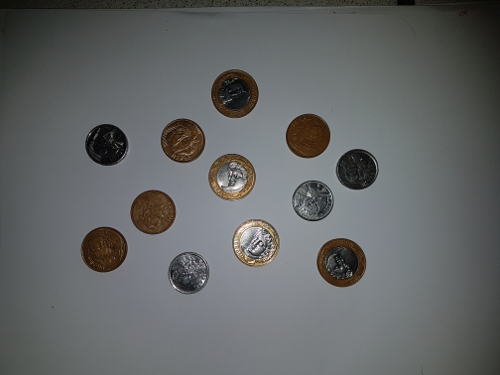
\includegraphics[width=0.5\textwidth]{gaussiano.jpg}
\caption{Imagem após filtragem para remoção de ruídos}
\label{fig:gaussiano}
\end{figure}

\begin{figure}[h]
\centering
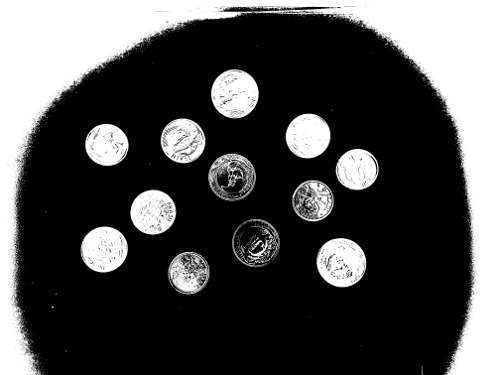
\includegraphics[width=0.5\textwidth]{binaria-otsu.jpg}
\caption{Limiarização da imagem através do método de Otsu}
\label{fig:binaria-otsu}
\end{figure}

\begin{figure}[h]
\centering
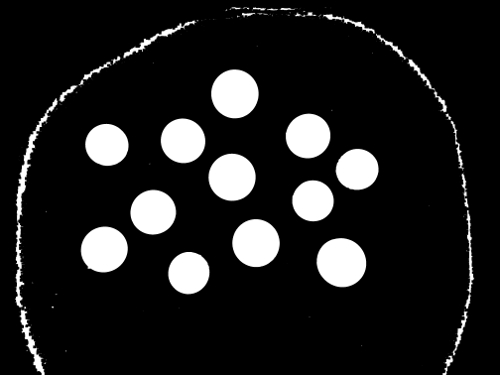
\includegraphics[width=0.5\textwidth]{fechamento-buracos.jpg}
\caption{Fechamento morfológico e remoção de buracos}
\label{fig:fechamento-buracos}
\end{figure}

\begin{figure}[h]
\centering
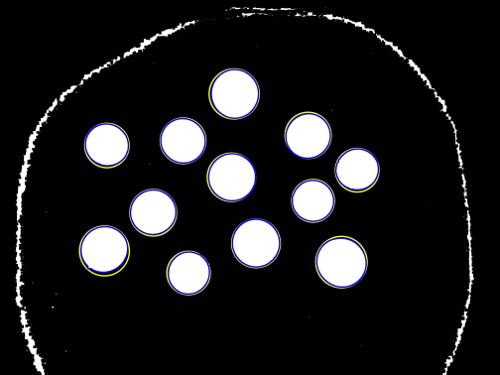
\includegraphics[width=0.5\textwidth]{circulos.jpg}
\caption{Detecção de círculos (contornos em azul e menor círculo em amarelo}
\label{fig:circulos}
\end{figure}

Apenas para facilitar o fim do processo, a Figura \ref{fig:resultado-segmentador} mostra a localização exata das moedas encontradas sob a imagem original (Figura \ref{fig:imagem-exemplo}).

\begin{figure}[h]
\centering
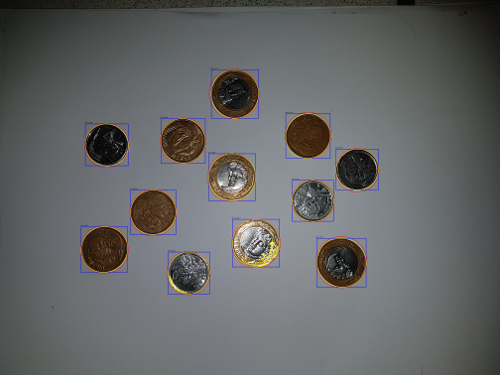
\includegraphics[width=0.5\textwidth]{resultado-segmentador.jpg}
\caption{Resultado do processo de segmentação}
\label{fig:resultado-segmentador}
\end{figure}

A partir dos retângulos em azul mostrado na Figura \ref{fig:resultado-segmentador}, são geradas imagens menores para cada um deles, de modo que todos os píxels fora do contorno são padronizados para cor branca em RGB. Um exemplo dessas imagens pode ser vista na Figura \ref{fig:moeda-individual}. Embora apareça uma pequena sombra em cinza ao redor da moeda, ela não foi suficiente para atrapalhar os resultados finais.

\begin{figure}[ht]
\centering
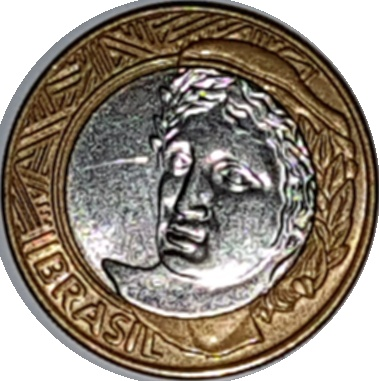
\includegraphics[width=0.5\textwidth]{moeda-individual.jpg}
\caption{Exemplo de moeda individual após segmentação}
\label{fig:moeda-individual}
\end{figure}


\begin{table*}[]
\centering
\begin{tabular}{@{}clcc@{}}
\toprule
\textbf{Moeda} & \textbf{Tipo}     & \textbf{Saída}                   & \textbf{Classificação} \\ \midrule
1              & R\$ 0,25 (número) & (1.00226, -0.997003, -1.0058)    & R\$ 0,25               \\
2              & R\$ 0,25 (número) & (0.992012, -0.997708, -1.00573)  & R\$ 0,25               \\
3              & R\$ 0,25 (face)   & (0.498484, -1.13654, -0.386701)  & R\$ 0,25               \\
4              & R\$ 0,25 (face)   & (1.00382, -1.00784, -0.990536)   & R\$ 0,25               \\
5              & R\$ 0,50 (número) & (-1.01978, 0.981279, -0.962827)  & R\$ 0,50               \\
6              & R\$ 0,50 (número) & (-1.00145, 1.02011, -1.00438)    & R\$ 0,50               \\
7              & R\$ 0,50 (face)   & (-0.981349, 0.976257, -0.997547) & R\$ 0,50               \\
8              & R\$ 0,50 (face)   & (-0.993451, 0.979165, -0.997587) & R\$ 0,50               \\
9              & R\$ 1,00 (número) & (-0.980049, -0.932487, 0.899731) & R\$ 1,00               \\
10             & R\$ 1,00 (número) & (-1.02751, -0.966398, 0.984723)  & R\$ 1,00               \\
11             & R\$ 1,00 (face)   & (-1.07407, -0.97125, 1.02219)    & R\$ 1,00               \\
12             & R\$ 1,00 (face)   & (-1.01076, -0.992155, 1.00249)   & R\$ 1,00               \\ \bottomrule
\end{tabular}
\caption{Resultado da validação}
\label{tab:resultado-validacao}
\end{table*}


\subsection{Calibrador}
\label{sec:calibrador}

Antes de usar o calibrador, o usuário do sistema precisa preparar três diretórios com exemplos dos três tipos de moeda já processadas pelo segmentador, para serem utilizadas como conjunto treinamento. É neste módulo onde o treinamento da rede neural artificial é feito e o resultado do treinamento é salvo em um arquivo de formato \textit{yml}, que será carregado durante a execução do validador e do contador. Os parâmetros da RNA foram:

\begin{itemize}  
\item Método de treinamento: \textit{Backpropagation}
\item Número de camadas escondidas: 2, cada uma com 32 neurônios.
\item Função de ativação: sigmoide simétrica, que varia de -1 a 1.
\item Número máximo de iterações: 10000
\item Erro mínimo de parada:  $10 ^ {-8}$.
\item Taxa de aprendizado: 0.1
\item Momentum: 0.1
\end{itemize}

Para o treinamento, foram utilizadas várias imagens além da própria Figura \ref{fig:imagem-exemplo}, o que produziu  20 imagens de R\$ 0,25, 20 de R\$ 0,50 e 20 de R\$ 1,00, sendo 10 da face e 10 da parte com o número para cada tipo, o que dá um total de 60 moedas. As 20 imagens de cada classe foram separadas em diretórios diferentes apenas por questão de organização. Como o conjunto treinamento e o número de entradas e saídas são pequenos, o treinamento da RNA durou em torno de 1 segundo, com pouco mais de 1300 iterações, para vários testes realizados.

\subsection{Validador}
\label{sec:validador}

Após a etapa de anterior de calibração, utiliza-se o programa validador, que utiliza outras imagens diferentes das utilizadas anteriormente para validar o resultado do treinamento. Seguindo a sequência do teste, foi criado um conjunto de validação com 4 moedas de cada tipo, sendo 2 da face e duas da parte com número, totalizando 12 moedas. Na Tabela \ref{tab:resultado-validacao}, pode-se notar que a taxa de acerto foi de 100\%, isto é, todas as moedas do conjunto de validação foram classificadas corretamente.

\subsection{Contador}
\label{sec:contador}

Com o processo de calibração do sistema concluído, finalmente o módulo contador, que é o produto final deste projeto, pode ser utilizado. Sua entrada consiste em uma imagem com várias moedas e sua saída é a soma do valor monetário de todas elas. Para realizar isso, este módulo utiliza tanto partes da técnica segmentação, para separar todas as moedas na imagem, quanto da calibração e validação, com o objetivo de identificar corretamente cada moeda encontrada. Ao fim, o sistema soma todos os valores das moedas e informa ao usuário.

Usando a mesma Figura \ref{fig:imagem-exemplo}, por fim, o programa conseguiu contar exatamente R\$ 7,00 na imagem, que é o valor exato da soma de 4 moedas de cada tipo. O tempo médio de execução do contador foi de 1,2 segundos. Na Figura  \ref{fig:resultado-contador}, é possível ver o resultado da contagem de moedas, bem como o tempo de execução do programa.

\begin{figure}[ht]
\centering
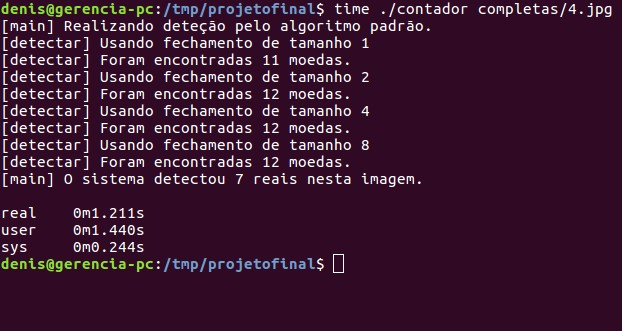
\includegraphics[width=0.5\textwidth]{resultado-contador.jpg}
\caption{Exemplo de moeda individual após segmentação}
\label{fig:resultado-contador}
\end{figure}


\section{Conclusão}
\label{sec:conclusao}

O programa de contagem de moedas valeu-se, primeiramente, da aquisição da imagem de moedas por meio de uma câmera de celular sob um fundo de cor branca. Essa estratégia acabou sendo escolhida para facilitar a detecção de moedas e posteriormente realizar a sua contagem, assim como a restrição de distância de 30 cm. Contudo, isso acabou tornando-se uma limitação do programa, pois seriam necessários muitos mais testes e eventuais modificações nos módulos para que o sistema operasse de forma correta em qualquer outra cor de fundo. 

A utilização dos conceitos de processamento digital de imagens aprendidas na disciplina de mesmo nome foram feitas na parte de segmentação das imagens. As técnicas utilizadas envolveram suavização da imagem utilizando o filtro gaussiano, utilização do método de Otsu na limiarização, fechamento morfológico através das operações de dilatação e erosão e também técnicas de rotulação. Nesse contexto, pôde-se perceber a importância do uso de técnicas simples de processamento de imagens que servem muito bem na resolução de problemas mais complexos, como os presentes neste projeto, e podem ser uma alternativa em relação aos métodos mais complexos utilizados nos artigos referenciados neste trabalho.

O uso de aprendizado de máquina, com rede neural artificial, foi necessária para realizar a classificação das moedas, devido a falhas de outros métodos que foram tentados, que se baseavam em algoritmos para detecção de semelhança entre a fotografia da moeda tirada e uma moeda modelo. Muitos deles não funcionavam bem quando a moeda estava rotacionada, movimento que é inerente a objetos circulares.
Após muitos experimentos, o uso de uma rede neural artificial revelou um grande sucesso nessa tarefa, com uma taxa de acerto de 100\% durante a validação.

Por fim, é importante ressaltar que o programa é apenas um protótipo devido aos alunos envolvidos terem estudado apenas uma parte introdutória do enorme ramo que é o de processamento digital de imagens, e também devido à limitação de tempo da disciplina. Portanto, ficam como objetivos futuros a melhoria do programa para identificar todos os tipos de moedas nacionais, para que ele possa ser mais rápido ao ponto de funcionar em tempo real através da captura de vídeo e possivelmente encontrar uma aplicação comercial local do programa desenvolvido, buscando facilitar a contagem de moedas por microempresários e dono de supermercados por um preço de aquisição baixo.  

\medskip

\bibliographystyle{ieeetr}
\bibliography{referencias.bib}


\end{document}



